\externaldocument{tech_eclipse_text}

\subsection{Visibility Calculations of Regions \label{vis}}
The visibility of each {\it region} is defined in Equation~\ref{vis_equation} to be the projected area along the line-of-sight modified by the limb-darkened intensity. This quantity varies as the star rotates. For example, flux from a {\it region} in the middle of the backside of the star will contribute nothing to the overall luminosity at that time. Half a rotation period later, that same {\it region} will be in the center of the front of the star and contribute a maximal amount of flux.

\begin{equation}
	V_{i,j} = \int_{\phi_1}^{\phi_2} \int_{\theta_1}^{\theta_2} \frac{I(\theta, \phi)}{I(0)} \sin^2{\theta}\cos{\phi}\,\mathrm{d}\theta \, \mathrm{d}\phi
	\label{vis_equation}
\end{equation}

The visibility equation is simply the integral of the dot product of the spherical surface element, d$A$ and the unit vector, $\hat{x}$, along the line-of-sight to the observer multiplied by the quadratic limb-darkening function provided in \citet{Claret2004}. $\phi_1$, $\phi_2$, $\theta_1$, and $\theta_2$ are in standard spherical coordinates and denote the angular limits of an individual {\it region}. For any type of {\it region} ({\it box}, {\it stripe}, or {\it longitude}), the limits change, but the equation remains the same. We solve this integral analytically and then substitute in the appropriate limits of integration.

To calculate the {\it longitude} visibilities, $\phi_1$ and $\phi_2$ are determined by the number of stripes, $n_s$, defined at the start of the program and then modified at each timestep based on the rotational phase of the star. The latitude limits, $\theta_1$ and $\theta_2$ are always 0 and $\pi$. For the {\it box} visibilities, the $\phi_1$ and $\phi_2$ limits are determined in the same way using the number of {\it boxes}, $n_b$. The latitude limits depend on the impact parameter and the radius of the planet such that $\theta_{1,2} = cos^{-1}(b \pm R_p)$. The {\it stripe} visibilities are calculated by subtracting the sum of the {\it box} visibilities in a given longitude range from the {\it longitude} visibility in the same range. Simplifying the calculation of the {\it stripe} visibilities is the primary reason for choosing the number of {\it boxes} to be an integer multiple of the number of {\it stripes}. The sum of all {\it stripe} and {\it box} visibilities at any timestep should be equal to 1.0 by definition except during a transit. 

When the planet passes in front of the star, the apparent brightness of the system diminishes by an amount related to the area of the planet. To incorporate this effect in the model flux, we modify the visibilities of the {\it boxes} that are blocked by the planet during a transit. At each timestep, we use the orbital properties of the planet and the rotational phase of the star to determine which {\it boxes} are blocked, either fully or partially, by the planet. Then we calculate the intersection of the planet with each of those {\it boxes} on the projected surface of the star. The resulting value is multiplied by the average limb-darkened intensity in the {\it box} and subtracted from its unocculted visibility. We approximate the occulted {\it box} by a cartesian rectangle intersecting a circle and use standard Euclidean geometry to determine the area of the sector that is contained within the {\it box}. To verify that the simplifying approximation that each of the {\it boxes} is a cartesian rectangle on the surface of the star is reasonable, we show a plot of our transit model over the \citet{MandelAgol2002} model generated from the same physical planet properties. The difference between the two models is less than $<*********************\%$. A typical {\it box} visibility curve is shown in Figure~\ref{box_vis}. In addition, we provide additional details about the visibility caluclations in Appendix~\ref{vis_appendix}. 

%Near the limbs, the curvature of the boxes as compared to the cartesian rectangles becomes more extreme, but the boxes are smaller and thus the absolute error is smaller. 

\begin{figure}[h]
	\centering
	\includegraphics[width=.5\textwidth]{images/transit_check.eps}
	\caption{Our model transit is shown on top while the Mandel \& Agol model is shown on the bottom. The difference between the two models is less than x\%.}
	\label{transit}
\end{figure}
*********Make this eps
\begin{figure}[h]
	\centering
	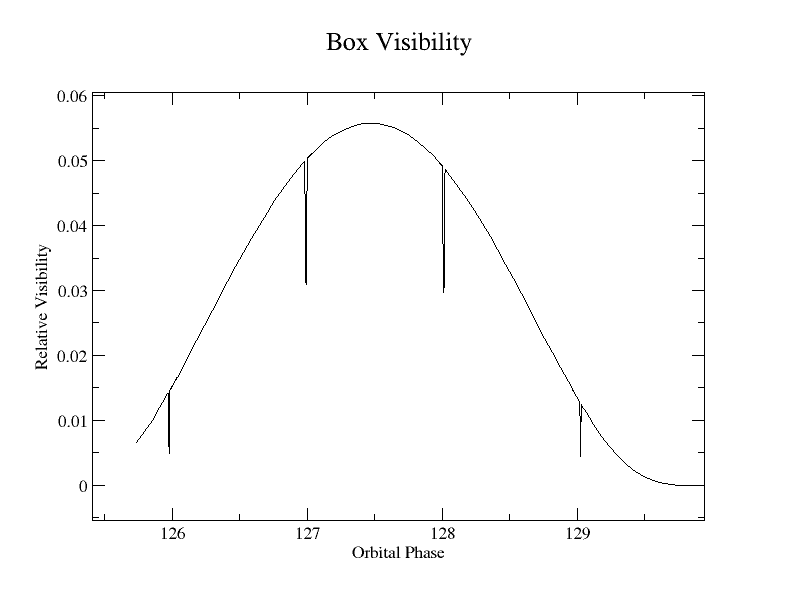
\includegraphics[width=.5\textwidth]{images/box_vis.eps}
	\caption{An example visibility curve for one {\it box}. This is "box 0", or the box whose left edge is on the left limb of the star at time 0 (the given epoch). This was generated for a system with the same parameters as Kepler-17, later shown in Section~\ref{validation}. $\theta_1$ and $\theta_2$ are $81.52^\circ$ and $96.4^\circ$ respectively.}
	\label{box_vis}
\end{figure}